\documentclass{article}
\usepackage[utf8]{inputenc}
\usepackage{xcolor}
\usepackage{listings}
\usepackage{graphicx}
\usepackage{caption}

\setlength{\topmargin}{-0.5in}
\setlength{\textheight}{9in}
\setlength{\oddsidemargin}{0.25in}
\setlength{\textwidth}{6in}

\title{Laboratorio 05 - Python}
\date{}

\lstset{
	backgroundcolor=\color{yellow},
	basicstyle=\ttfamily,
	frame=single,
	columns=fullflexible,
	breaklines=true
}

\begin{document}
	
	\maketitle
	
	\begin{tabular}{|p{\dimexpr\linewidth/3-2\tabcolsep}|p{\dimexpr\linewidth/3-2\tabcolsep}|p{\dimexpr\linewidth/3-2\tabcolsep}|}
		\hline\color{red}
		Profesor & \color{red}Escuela & \color{red}Asignatura \\
		\hline
		M.Sc. Ing. Richart Smith Escobedo Quispe & Escuela Profesional de Ingeniería de Sistemas & Programación Web II \\
		\hline
	\end{tabular}
	
	\vspace{10pt}
	
	\begin{tabular}{|p{\dimexpr\linewidth/3-2\tabcolsep}|p{\dimexpr\linewidth/3-2\tabcolsep}|p{\dimexpr\linewidth/3-2\tabcolsep}|}
		\hline\color{red}
		Laboratorio & \color{red}Tema & \color{red}Duración \\
		\hline
		05 & Python & 04 horas \\
		\hline
	\end{tabular}
	
	\vspace{10pt}
	
	\begin{tabular}{|p{\dimexpr\linewidth/3-2\tabcolsep}|p{\dimexpr\linewidth/3-2\tabcolsep}|p{\dimexpr\linewidth/3-2\tabcolsep}|}
		\hline
		\color{red}Semestre & \color{red}Fecha de inicio & \color{red}Fecha de entrega \\
		\hline
		2024 - A & 27 Mayo 2024 & 31 Mayo 2024 \\
		\hline
	\end{tabular}
	
	\section*{Ejercicios Propuestos}
	En esta tarea usted pondrá en práctica sus conocimientos de programación en Python para dibujar un tablero de Ajedrez.
	La parte gráfica ya está programada, usted sólo tendrá que concentrarse en las estructuras de datos subyacentes.
	Estos objetos estarán disponibles importando la biblioteca: chessPictures y estarán internamente representados con arreglos de strings que podrá revisar en el archivo pieces.py
	La clase Picture tiene un sólo atributo: el arreglo de strings img, el cual contendrá la representación en caracteres de la figura que se desea dibujar.
	La clase Picture ya cuenta con una función implementada, no debe modificarla, pero si puede usarla para implementar sus otras funciones:\\
	\_invColor: recibe un color como un caracter de texto y devuelve su color negativo, también como texto, deberá revisar el archivo colors.py para conocer los valores negativos de cada caracter.\\La clase Picture contará además con varios métodos que usted deberá implementar:
	
	\begin{itemize}
		\item verticalMirror: Devuelve el espejo vertical de la imagen
		\item horizontalMirror: Devuelve el espejo horizontal de la imagen
		\item negative: Devuelve un negativo de la imagen
		\item join: Devuelve una nueva figura poniendo la figura del argumento al lado derecho de la figura actual
		\item up: Devuelve una nueva figura poniendo la figura recibida como argumento, encima de la figura actual
		\item under: Devuelve una nueva figura poniendo la figura recibida como argumento, sobre la figura actual
		\item horizontalRepeat: Devuelve una nueva figura repitiendo la figura actual al costado la cantidad de veces que indique el valor de n
		\item verticalRepeat: Devuelve una nueva figura repitiendo la figura actual debajo, la cantidad de veces que indique el valor de n
	\end{itemize}
	
	Tenga en cuenta que para implementar todos estos métodos, sólo deberá trabajar sobre la representación interna de un Picture, es decir su atributo img.
	Para dibujar una objeto Picture bastará importar el método draw de la biblioteca interpreter y usarlo de la siguiente manera:
	
	\begin{lstlisting}
		$ python3
		Python 3.9.2 (default, Feb 28 2021, 17:03:44)
		[GCC 10.2.1 20210110] on linux
		Type "help", "copyright", "credits" or "license" for more information.
		>>> from chessPictures import *
		>>> from interpreter import draw
		pygame 1.9.6
		Hello from the pygame community. https://www.pygame.org/contribute.html
		>>> draw(rock)
	\end{lstlisting}
	
	Para resolver los siguientes ejercicios sólo está permitido usar ciclos, condicionales, definición de listas por comprensión, sublistas, map, join, (+), lambda, zip, append, pop, range.\\
	Implemente los métodos de la clase Picture. Se recomienda que implemente la clase picture por etapas, probando realizar los dibujos que se muestran en la siguiente preguntas.\\
	Usando únicamente los métodos de los objetos de la clase Picture dibuje las siguientes figuras (invoque a draw)
	
	\section*{Solución de los ejercicios propuestos}
	Para la resolución del segundo laboratorio se creó el siguiente repositoiro en GitHub:\\    
	https://github.com/LuisArocutipa/pw2-24a/tree/main/Lab0 
	\\Primero implementamos los archivos necesarios (colors.py, interpreter.py, picture.py, pieces.py y chessPictures.py) a la carpeta donde vamos a trabajar.
	\\Comenzamos completando las funciones de la clase Picture.py:
	\begin{itemize}
		\item verticalMirror: 
		\begin{lstlisting}
		def verticalMirror(self):
			vertical = []
			for value in self:
				inv = ""
				for x in value:
					inv = x + inv
				vertical.append(inv)
			return Picture(vertical)
		\end{lstlisting}
		\item horizontalMirror:
		\begin{lstlisting}
		def horizontalMirror(self):
			horizontal = []
			for value in self:
				horizontal.insert(0, value)
			return Picture(horizontal)
		\end{lstlisting}
		\item negative:
		\begin{lstlisting}
		def negative(self):
			negative = []
			for value in self.img:
				new = ""
				for x in value:
					new += self._invColor(x)
				negative.append(new)
			return Picture(negative))
		\end{lstlisting}
		\item join:
		\begin{lstlisting}
		def join(self, p):
			joinAr = []
			for value in range(len(self.img)):
				joinAr.append(self.img[value] + p.img[value])
			return Picture(joinAr)
		\end{lstlisting}
		\item up:
		\begin{lstlisting}
		def up(self, p):
			upAr = self.img + p.img
			return Picture(upAr)
		\end{lstlisting}
		\item under:
		\begin{lstlisting}
		def under(self, p):
			underAr = []
			for value in range(len(self.img)):
				new = ""
				for x in range(len(self.img)):
					if p.img[value][x] == " ":
						new += self.img[value][x]
					else:
						new += p.img[value][x]
				underAr.append(new)
			return Picture(underAr)
		\end{lstlisting}
		\item horizontalRepeat:
		\begin{lstlisting}
		def horizontalRepeat(self, n):
			horizontalAr = []
			for value in self.img:
				horizontalAr.append(value*n)
			return Picture(horizontalAr)
		\end{lstlisting}
		\item verticalRepeat:
		\begin{lstlisting}
		def verticalRepeat(self, n):
			verticalAr = self.img*n
			return Picture(verticalAr)
		\end{lstlisting}
	\end{itemize}
	Luego se creó un archivo .py para cada ejercicio y se se importó las funciones y objetos necesarios para el uso específico en cada problema
	\begin{itemize}
		\item Ejercicio 01:
		\begin{lstlisting}
	from interpreter import draw
	from chessPictures import *
			
	draw(knight.join(knight.negative()).up(knight.negative().join(knight)))
		\end{lstlisting}
		\begin{figure}[h]
			\centering
			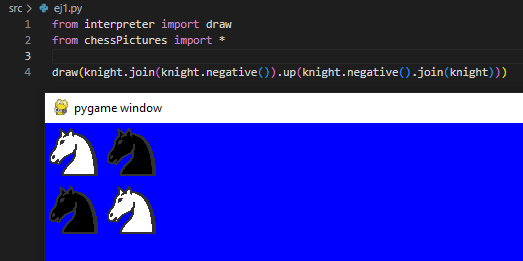
\includegraphics[width=0.5\textwidth]{Imagenes/4e1.png}
			\caption{Captura del ejercicio 1}
		\end{figure}
		\item Ejercicio 02:
		\begin{lstlisting}
	from interpreter import draw
	from chessPictures import *
			
	draw(knight.join(knight.negative()).up(knightVertical.negative().join(knightVertical)))
		\end{lstlisting}
		\begin{figure}[h]
			\centering
			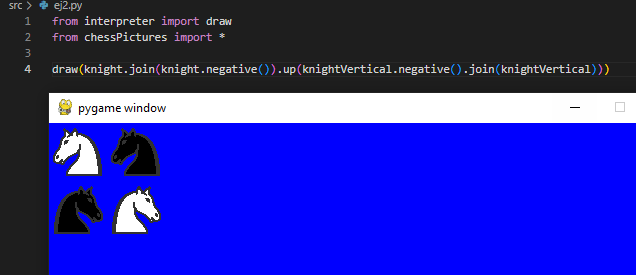
\includegraphics[width=0.5\textwidth]{Imagenes/4e2.png}
			\caption{Captura del ejercicio 2}
		\end{figure}
		\item Ejercicio 03:
		\begin{lstlisting}
	from interpreter import draw
	from chessPictures import *
			
	draw(queen.horizontalRepeat(4))
		\end{lstlisting}
		\begin{figure}[h]
			\centering
			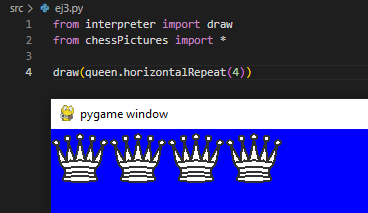
\includegraphics[width=0.5\textwidth]{Imagenes/4e3.png}
			\caption{Captura del ejercicio 3}
		\end{figure}
		\item Ejercicio 04:
		\begin{lstlisting}
	from interpreter import draw
	from chessPictures import *
			
	draw(square.join(square.negative()).horizontalRepeat(4))
		\end{lstlisting}
		\begin{figure}[h]
			\centering
			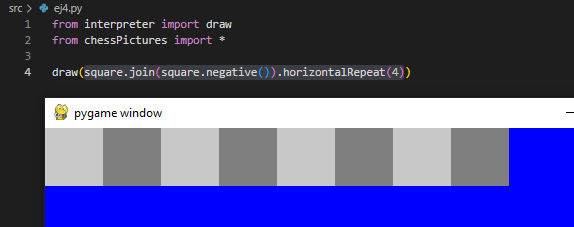
\includegraphics[width=0.5\textwidth]{Imagenes/4e4.png}
			\caption{Captura del ejercicio 4}
		\end{figure}
		\item Ejercicio 05:
		\begin{lstlisting}
	from interpreter import draw
	from chessPictures import *
			
	draw(square.negative().join(square).horizontalRepeat(4))
		\end{lstlisting}
		\begin{figure}[h]
			\centering
			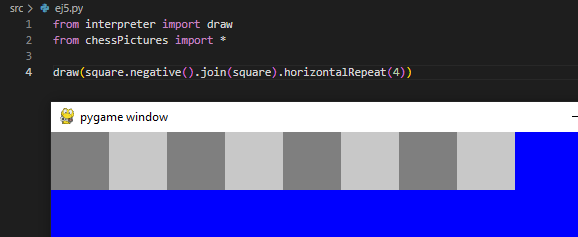
\includegraphics[width=0.5\textwidth]{Imagenes/4e5.png}
			\caption{Captura del ejercicio 5}
		\end{figure}
		\item Ejercicio 06:
		\begin{lstlisting}
	from interpreter import draw
	from chessPictures import *
			
	draw(square.join(square.negative()).horizontalRepeat(4).up(square.negative().join(square).horizontalRepeat(4)).verticalRepeat(2))
		\end{lstlisting}
		\begin{figure}[h]
			\centering
			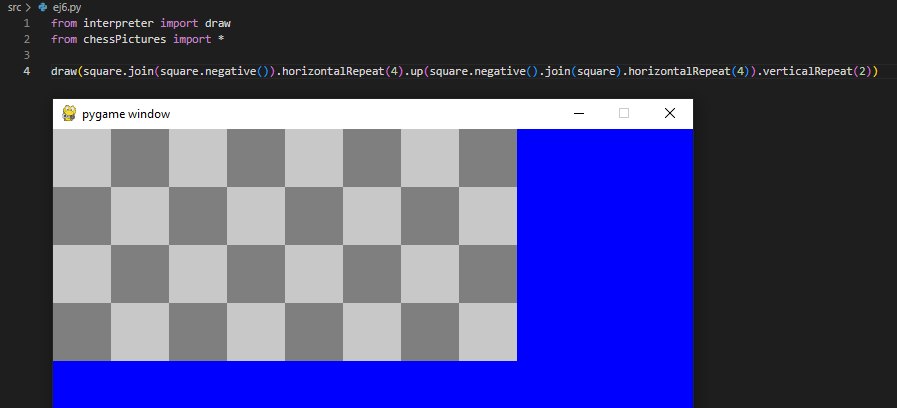
\includegraphics[width=0.5\textwidth]{Imagenes/4e6.png}
			\caption{Captura del ejercicio 6}
		\end{figure}
		
		\item Ejercicio 07:
		\begin{lstlisting}
	from interpreter import draw
	from chessPictures import *
			
	draw(square.under(rock.negative()).join(square.negative().under(knight.negative())).join(square.under(bishop.negative())).join(square.negative().under(queen.negative()))
	.join(square.under(king.negative())).join(square.negative().under(bishop.negative())).join(square.under(knight.negative())).join(square.negative().under(rock.negative()))
	.up(square.negative().under(pawn.negative()).join(square.under(pawn.negative())).horizontalRepeat(4))
	.up(square.join(square.negative()).horizontalRepeat(4).up(square.negative().join(square).horizontalRepeat(4)).verticalRepeat(2))
	.up(square.under(pawn).join(square.negative().under(pawn)).horizontalRepeat(4))
	.up(square.negative().under(rock).join(square.under(knight)).join(square.negative().under(bishop)).join(square.under(queen))
	.join(square.negative().under(king)).join(square.under(bishop)).join(square.negative().under(knight)).join(square.under(rock))))
		\end{lstlisting}
		\begin{figure}[h]
			\centering
			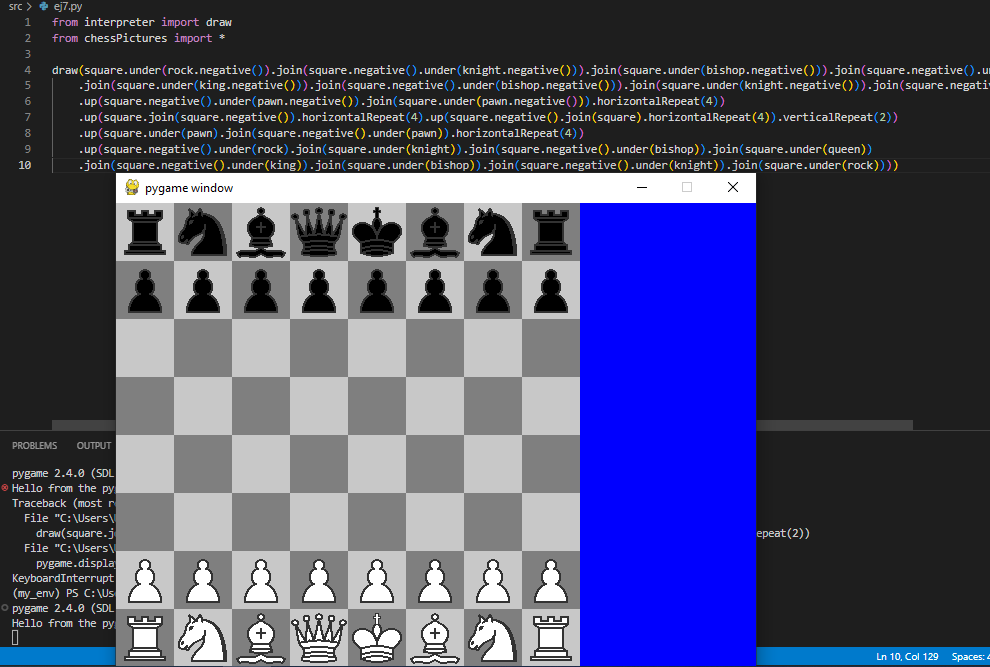
\includegraphics[width=0.5\textwidth]{Imagenes/4e7.png}
			\caption{Captura del ejercicio 7}
		\end{figure}
	\end{itemize}
	
	\section*{Pregunta}
	\begin{enumerate}
		\item Explique: ¿Para qué sirve el directorio pycache?
		\\La función principal del directorio "pycache" es proporcionar un lugar específico para almacenar los archivos de bytecode generados por el intérprete de Python. Almacenar estos archivos en un directorio separado ayuda a mantener organizado el árbol de directorios del proyecto y evita la saturación del directorio principal con archivos ".pyc".
	\end{enumerate}
	
\end{document}
